\documentclass{article}
\usepackage[T1]{fontenc}
\usepackage{lmodern}
\usepackage{graphicx}
\usepackage{amsmath,amssymb}
\usepackage[a4paper,margin=2cm]{geometry}
\usepackage[absolute,overlay]{textpos}
\setlength{\TPHorizModule}{1mm}
\setlength{\TPVertModule}{1mm}
\usepackage[indonesian]{babel}
\usepackage{hyperref}
\setlength{\emergencystretch}{2em}
% unit: Halaman 27

\begin{document}

% === Halaman 27 (llm) ===

Jika diteruskan untuk $x = 4, 5, \dots, 10$, diperoleh tabel sebagai berikut :

\vspace{10mm}

Jadi, titik-titik yang terdapat pada kurva eliptik adalah 12, yaitu:
(2, 4), (2, 7), (3, 5), (3, 6), (5, 2), (5, 9), (7, 2), (7, 9), (8, 3), (8, 8), (10, 2), (10, 9)

\vspace{5mm}

Jika ditambah dengan titik O di infinity, maka titik-titik pada kurva eliptik membentuk grup dengan $n = 13$ elemen.

\vspace{10mm}

\begin{flushright}
\textcolor{red}{Sumber: Andreas Steffen, \\
Elliptic Curve Cryptography}
\end{flushright}

% deskripsi: Tabel perhitungan nilai x, y^2, y_{1,2}, P(x,y), dan P'(x,y) untuk kurva eliptik dengan beberapa coretan tangan penanda.
% bbox normalisasi: [0.1800, 0.2200, 0.4700, 0.8300]
\begin{textblock*}{60.90mm}(37.80mm,65.34mm)
\noindent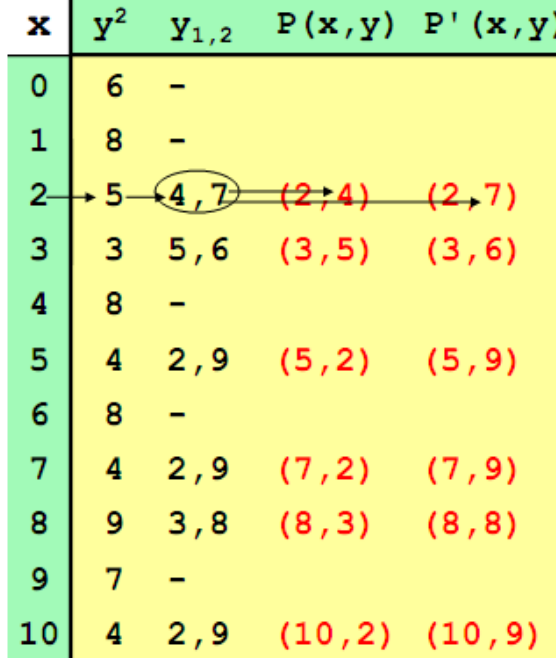
\includegraphics[width=60.90mm,height=181.17mm]{../../images/llm/page_027_img_01.png}%
\end{textblock*}

\end{document}
